\section{C/C++ Binding}
\label{sec:C}

COMPSs provides a binding for C and C++ applications. The new C++ version in the current release 
comes with support for objects as task parameters and the use of class methods as tasks.

\subsection{Programming Model}

\subsubsection{Task Selection}
As in Java the user has to provide a task selection by means of an interface. In this case 
the interface file has the same name as the main application file plus the suffix ``idl'', 
i.e. Matmul.idl, where the main file is called Matmul.cc.

\begin{lstlisting}[language=C++]
interface Matmul
{
      // C functions
      void initMatrix(inout Matrix matrix,
                      in int mSize,
                      in int nSize,
                      in double val);
                      
      void multiplyBlocks(inout Block block1,
                          inout Block block2,
                          inout Block block3);
                          
      // C++ class methods
      void Block::multiply(in Block block1,
                           in Block block2);
                           
      static Matrix Matrix::init(in int mSize,
                                 in int bSize,
                                 in double val);
};
\end{lstlisting}

The syntax of the interface file is shown in the previous code. Tasks can be declared as classic 
C function prototypes, this allow to keep the compatibility with standard C applications. 
In the example, initMatrix and multiplyBlocks are functions declared using its prototype, 
like in a C header file, but this code is C++ as they have objects as parameters (objects of 
type Matrix, or Block).

A class method can be also a task, and it is declared using its signature. In the example, 
Block::multiply and Matrix::init are class methods. In this example, C functions encapsulates 
object method calls, as we will see later.

The grammar for the interface file is:

\begin{lstlisting}[language=bash]
["static"] return-type task-name ( parameter {, parameter }* );

return-type = "void" | type

ask-name = <qualified name of the function or method>

parameter = direction type parameter-name

direction = "in" | "out" | "inout"

type = "char" | "string" | "int" | "short" | "long"
    | "float" | "double" | "boolean" | "File" | class-name

class-name = <qualified name of the class>
\end{lstlisting}

       
\subsubsection{Value and Object return}
The binding allows returning a value (void, int, long, float, etc.) or an object from a 
function or method. In C/C++ the default policy is to make a copy of the value or object when it is returned [A = foo();], 
and this copy (A) is a new position in memory whom reference or address is not possible to know before 
the return statement. As the COMPSs runtime cannot know such reference before returning from the task execution (foo) it must do a 
synchronization before the return statement for the correct value to be copied when returning. 
This is called an explicit synchronization.

Alternatively, the return of a value or an object can be done also by mean of an out or inout parameter, 
and no explicit synchronization is needed because the reference is passed to the binding in this case 
using the \& operator [foo(\&A);].

\subsubsection{Main Program}
The next listing includes an example of matrix multiplication written in C++.

\begin{lstlisting}[language=C++]
#define %*{\bf DEBUG\_BINDING }*)
#include %*{\bf "Matmul.h" }*)
#include "Matrix.h"
#include ""Block.h"
int N; //MSIZE
int M; //BSIZE
double val;
int main(int argc, char **argv)
{
      Matrix A;
      Matrix B;
      Matrix C;

       N = atoi(argv[1]);
       M = atoi(argv[2]);
      val = atof(argv[3]);

      %*{\bf compss\_on(); }*)

      A = Matrix::init(N,M,val);

      initMatrix(&B,N,M,val);
      initMatrix(&C,N,M,0.0);

      cout << "Waiting for initialization...\n";

      %*{\bf compss\_wait\_on(B); }*)
      %*{\bf compss\_wait\_on(C); }*)

      cout << "Initialization ends...\n";
 
      C.multiply(A, B);

      %*{\bf compss\_off(); }*)
      return 0;
}
\end{lstlisting}

The developer has to take into account the following rules:
\begin{enumerate}
 \item The directive {\bf DEBUG\_BINDING} can be defined if we need debug information from the binding.
 \item A header file with the same name as the main file must be included, in this case {\bf Matmul.h}. 
       This header file is automatically generated by the binding and it contains other includes and 
        type-definitions that are required.
 \item A call to the {\bf compss\_on} binding function is required to turn on the COMPSs runtime.
 \item As in C language, out or inout parameters should be passed by reference by means of the ``{\bf \&}'' 
       operator before the parameter name.
 \item Synchronization on a parameter can be done calling the {\bf compss\_wait\_on} binding function. 
       The argument of this function must be the variable or object we want to synchronize.
 \item There is an {\bf implicit synchronization} in the init method of Matrix. It is not possible to 
       know the address of ``A'' before exiting the method call and due to this it is necessary to synchronize 
       before for the copy of the returned value into ``A'' for it to be correct.
 \item A call to the {\bf compss\_off} binding function is required to turn off the COMPSs runtime.
\end{enumerate}


\subsubsection{Functions file}
The implementation of the tasks in a C or C++ program has to be provided in a functions file. 
Its name must be the same as the main file followed by the suffix ``-functions''. In our case Matmul-functions.cc.

\begin{lstlisting}[language=C++]
#include "Matmul.h"
#include "Matrix.h"
#include "Block.h"

void initMatrix(Matrix *matrix,int mSize,int nSize,double val){
     *matrix = Matrix::init(mSize, nSize, val);
}

void multiplyBlocks(Block *block1,Block *block2,Block *block3){
     block1->multiply(*block2, *block3);
}
\end{lstlisting}

In the previous code, class methods have been encapsulated inside a function. 
This is useful when the class method returns an object or a value and we want to avoid the explicit 
synchronization when returning from the method.

\subsubsection{Additional source Files}
Other source files needed by the user application must be placed under the directory ``{\bf src}''.
In this directory the programmer must provide a {\bf Makefile} that compiles such source files in the proper way. 
When the binding compiles the whole application it will enter into the src directory and execute the Makefile.
 
It generates two libraries, one for the master application and another for the worker application. 
The directive COMPSS\_MASTER or COMPSS\_WORKER must be used in order to compile the source files for each type of library. 
Both libraries will be copied into the lib directory where the binding will look for them when generating the master and worker applications.

\subsubsection{Class Serialization}
In case of using an object as method parameter, as callee or as return of a call to a function, the object has to be serialized. The serialization method has to be provided inline in the header file of the object's class by means of the ``{\bf boost}'' library. The next listing contains an example of serialization for two objects of the Block class.

\begin{lstlisting}[language=C++]
#ifndef BLOCK_H
#define BLOCK_H

#include    <vector>
#include    <boost/archive/text_iarchive.hpp>
#include    <boost/archive/text_oarchive.hpp>
#include    <boost/serialization/serialization.hpp>
#include    <boost/serialization/access.hpp>
#include    <boost/serialization/vector.hpp>

using namespace std;
using namespace boost;
using namespace serialization;

class Block {
public:
    Block(){};

    Block(int bSize);
       
    static Block *init(int bSize, double initVal);
        
    void multiply(Block block1, Block block2);
        
    void print();

private:
    int M;
    std::vector< std::vector< double > > data;
        
    %*{\bf friend class::serialization::access; }*)
    %*{\bf template$<$class Archive$>$ }*)
    %*{\bf void serialize(Archive \& ar, const unsigned int version) \{ }*)
        %*{\bf ar \& M; }*)
        %*{\bf ar \& data; }*)
    %*{\bf \} }*)
};

#endif
\end{lstlisting}

For more information about serialization using ``boost'' visit the related documentation at \url{www.boost.org}.


\subsubsection{Method - Task}

A task can be a C++ class method. A method can return a value, modify the \textit{this} object, or modify a parameter.

If the method has a return value there will be an implicit synchronization before exit the method, 
but for the \textit{this} object and parameters the synchronization can be done later after the method has finished.

This is because the \textit{this} object and the parameters can be accessed inside and outside the method, but for the 
variable where the returned value is copied to, it can’t be known inside the method.

\begin{lstlisting}[language=C++]
#include "Block.h"

Block::Block(int bSize) {
       M = bSize;
       data.resize(M);
       for (int i=0; i<M; i++) {
              data[i].resize(M);
       }
}

Block *Block::init(int bSize, double initVal) {
       Block *block = new Block(bSize);
       for (int i=0; i<bSize; i++) {
              for (int j=0; j<bSize; j++) {
                     block->data[i][j] = initVal;
              }
       }
       return block;
}

#ifdef COMPSS_WORKER

void Block::multiply(Block block1, Block block2) {
       for (int i=0; i<M; i++) {
              for (int j=0; j<M; j++) {
                     for (int k=0; k<M; k++) {
                            data[i][j] += block1.data[i][k] * block2.data[k][j];
                     }
              }
       }
       this->print();
}

#endif

void Block::print() {
       for (int i=0; i<M; i++) {
              for (int j=0; j<M; j++) {
                     cout << data[i][j] << " ";
              }
              cout << "\r\n";
       }
}
\end{lstlisting}

\subsection{Application Compilation}
To compile the user application with the C/C++ binding  the ``{\bf buildapp}'' command the user has to be executed in the directory of the main application code; 
the name of the application has to be passed as argument to this script, in this case \textit{Matmul}.

\begin{lstlisting}[language=bash]
user@localhost:~/matmul_objects$ buildapp Matmul

Building application...

g++ -DCOMPSS_MASTER -g -I. -I/opt/COMPSs/Runtime/bindings/c/include -I/opt/COMPSs/Runtime/bindings/bindings-common/include -c Block.cc Matrix.cc ar rvs libmaster.a Block.o Matrix.o

g++ -DCOMPSS_WORKER -g -I. -I/opt/COMPSs/Runtime/bindings/c/include -I/opt/COMPSs/Runtime/bindings/bindings-common/include -c Block.cc Matrix.cc ar rvs libworker.a Block.o Matrix.o

Building all:

Building Master...

g++ -g -O2 -o Matmul Matmul-empty.o Matmul-stubs.o Matmul.o -L../../lib -lmaster -L/usr/lib/jvm/java-6-openjdk-amd64/jre/lib/amd64/server -ljvm -ldl -L/opt/COMPSs/Runtime/bindings/c/../bindings-common/lib -lbindings_common -L/opt/COMPSs/Runtime/bindings/c/lib -lcbindings -lboost_iostreams -lboost_serialization

Building Worker...

g++ -g -O2 -o Matmul-worker Matmul-worker.o Matmul-functions.o -L../../lib -lworker -ldl -lboost_iostreams -lboost_serialization -L/opt/COMPSs/Runtime/bindings/c/lib

Command succesful.
\end{lstlisting}

\emph{[The previous output has been cut for simplicity]}


\subsection{Application Execution}

The following environment variables must be defined before executing a COMPSs C/C++ application:
            
JAVA\_HOME: Java JDK installation directory (e.g. /usr/lib/jvm/java-7-openjdk/)

After compiling the application, two directories, master and worker, are generated. 
The master directory contains a binary called as the main file, which is the master application, in our 
example is called Matmul. The worker directory contains another binary called as the main file followed 
by the suffix ``-worker'', which is the worker application, in our example is called Matmul-worker.

The \textit{runcompss} script has to be used to run the application:

\begin{lstlisting}[language=bash]
compss@bsc:~$ runcompss \
                 --lang=c \
                 -g \
                 /home/compss/workspace_c/matmul_objects/master/Matmul 3 4 2.0
\end{lstlisting}

The completelist of options of the runcompss command is available in the \textit{COMPSs User Manual: Application
Execution} at \url{http://compss.bsc.es} . 

\subsection{Execution Graph}
Figure 1 depicts the execution graph for the Matmul application in its object version with 3x3 blocks matrices, each one containing a 4x4 matrix of doubles.
Each block in the result matrix accumulates three block multiplications, i.e. three multiplications of 4x4 matrices of doubles.

The light blue circle corresponds to the initialization of matrix ``A'' by means of a method-task and it has 
an implicit synchronization inside. The dark blue circles correspond to the other two initializations by 
means of function-tasks; in this case the synchronizations are explicit and must be provided by the developer after the 
task call. Both implicit and explicit synchronizations are represented as red circles.

Each green circle is a partial matrix multiplication of a set of 3. One block from matrix ``A'' and the 
correspondent one from matrix ``B''. The result is written in the right block in ``C'' that accumulates 
the partial block multiplications. Each multiplication set has an explicit synchronization. 
All green tasks are method-tasks and they are executed in parallel.

\begin{figure}[ht!]
  \centering
    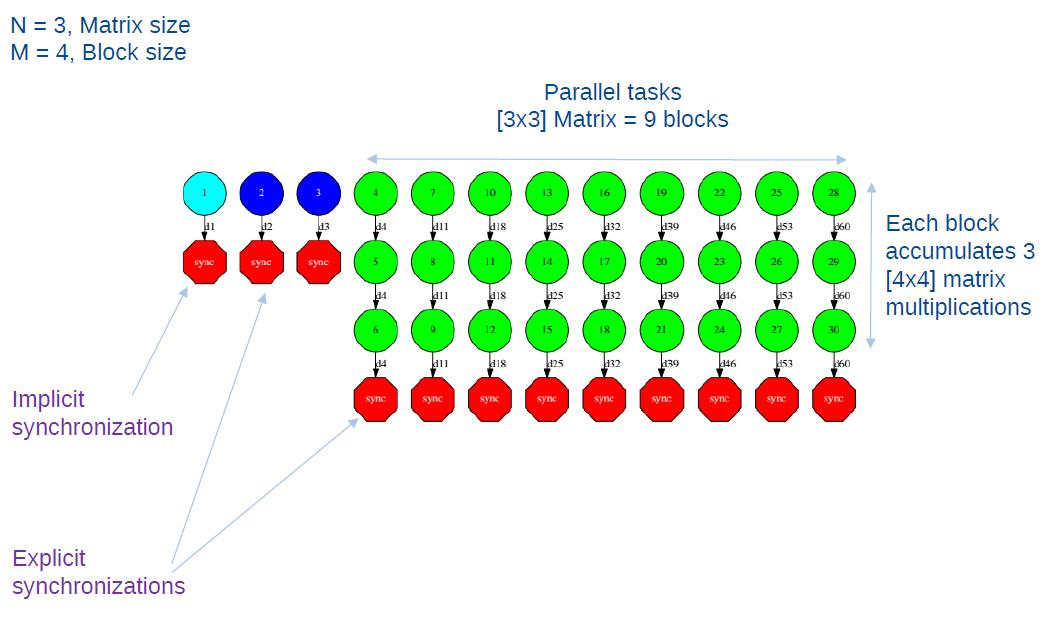
\includegraphics[width=1.0\textwidth]{./Sections/4_C/Figures/matmul.jpeg}
    \caption{Matmul Execution Graph.}
    %\label{fig:BLAST_workflow}
\end{figure}
